\documentclass{article}

\usepackage[utf8]{inputenc}
\usepackage{amsmath}
\usepackage{booktabs}
\usepackage{geometry}
\usepackage{pgfplots}
\pgfplotsset{compat=1.18}

\geometry{margin=1in}

\title{RLM vs LLM Evaluation}
\author{Abhigyan Shekhar}
\date{}

\begin{document}

\maketitle

\section{Evaluation}

This section summarizes what we found when comparing two ways of getting things done: direct LLM prompting and RLM-based execution. We evaluated five tasks and compared accuracy, latency, and token usage across both approaches.

\subsection{Experimental Scope}

We tested five tasks:

\begin{itemize}
    \item Reasoning (Battle of the Bastards)
    \item Long-context retrieval (AuthProxy)
    \item Structured extraction (clinical trial)
    \item Planning (30-day product launch)
    \item PDF question answering (Cersei/Ned quote)
\end{itemize}

For each task we tried two approaches:

\begin{itemize}
    \item Direct LLM calls (Gemini 2.5 Flash Lite)
    \item RLM-based runs with iteration, REPL execution, and optional recursion
\end{itemize}

We measured:

\begin{itemize}
    \item Answer correctness
    \item Latency (execution and wall time)
    \item Token usage (input/output totals)
\end{itemize}

\subsection{Task-by-Task Findings}

\subsubsection{1. Short Reasoning Task}

The short reasoning task was to identify a character and a decisive ally.

The direct LLM usually produced the answer in about 1 second using around 270 tokens.

The RLM approach also produced correct answers in some runs, but it took between 6 and 9 seconds and used between 3{,}700 and 13{,}000 tokens.

One RLM run failed and produced an unrelated answer to a different prompt.

\textbf{Finding:} RLM did not improve correctness on this task. It made the process slower, more expensive in tokens, and more failure-prone.

\subsubsection{2. Long-Context Retrieval (AuthProxy)}

This task required extracting answers from a long document.

The direct LLM answered all questions correctly in around 1.46 seconds using around 1{,}512 tokens.

The RLM run took around 13 seconds, used around 11{,}000 tokens, and still produced an incorrect final answer.

\textbf{Finding:} The extra computation did not improve retrieval quality. In practice, it performed worse despite higher cost.

\subsubsection{3. Structured Extraction (Clinical Trial)}

This task required extracting multiple fields together with an exact sentence from a clinical-trial document.

The direct LLM produced a structured output in around 1.96 seconds using around 2{,}124 tokens.

The RLM output was only partially correct. It missed one required field (Q4) even though it used around 11{,}771 tokens and took around 15 seconds.

\textbf{Finding:} RLM preserved some structure but failed on completeness, which made it less reliable despite higher compute usage.

\subsubsection{4. Planning Task}

This task was to generate a 30-day launch plan.

Both approaches produced plans with dependencies, risks, and structured timelines.

The direct LLM completed the task in around 8 seconds using around 2{,}144 tokens.

The RLM run took around 20 seconds and used around 11{,}216 tokens.

\textbf{Finding:} Output quality was roughly tied, but the direct LLM remained far more efficient in both time and token cost.

\subsubsection{5. PDF Question Answering (Cersei Task)}

This task was to locate a quote from a source document.

The direct LLM produced an answer with the wrong speaker, but still finished in around 36 seconds using around 195{,}109 tokens.

The RLM run failed badly, including:

\begin{itemize}
    \item repeated looping over incorrect guesses
    \item tool misuse
    \item runtime errors (\texttt{NameError})
    \item outputting the literal string \texttt{result}
\end{itemize}

Further investigation showed that RLM could not reliably read from file paths or perform autonomous retrieval. However, when it was constrained to operate directly on the provided context, avoid \texttt{llm\_query}, and use explicit Python string operations, it successfully extracted the correct quote.

\textbf{Finding:} RLM can succeed in long-context extraction under strong constraints, but autonomous retrieval and strategy selection were not shown to be reliable.

\subsection{Cross-Task Observations}

\begin{itemize}
    \item \textbf{Speed:} Direct LLM execution was faster across all tasks. The gap widened for RLM runs involving iteration or recursion.
    \item \textbf{Token Usage:} Direct LLM prompting was consistently more token-efficient across all tasks except the PDF case, where full-document upload dominated token usage. Even there, RLM used fewer tokens but still performed worse and was much slower.
    \item \textbf{Reliability:} Direct LLM runs were stable and consistently produced usable outputs. RLM showed multiple failure modes:
    \begin{itemize}
        \item task drift
        \item incomplete outputs
        \item runtime errors
        \item looping behavior
        \item incorrect final formatting
    \end{itemize}
\end{itemize}

\subsection{Key Observations}

Across all tasks, RLM consistently incurred significantly higher token usage and latency compared to direct LLM prompting. However, this increase in computational cost did not translate into consistent improvements in accuracy or output quality.

In several cases, including long-context retrieval and structured extraction, RLM produced worse results despite higher resource consumption. These findings highlight a mismatch between the theoretical advantages of recursive decomposition and practical performance.

\section{Quantitative Comparison}

\subsection{Token Usage Table}

\begin{center}
\begin{tabular}{|l|c|c|}
\hline
Task & LLM Tokens & RLM Tokens \\
\hline
Reasoning & 270 & 9650 \\
AuthProxy & 1512 & 11003 \\
Clinical & 2124 & 11771 \\
Planning & 2144 & 11216 \\
PDF & 195109 & 141006 \\
\hline
\end{tabular}
\end{center}

\subsection{Accuracy Table}

\begin{center}
\begin{tabular}{|l|c|c|}
\hline
Task & LLM & RLM \\
\hline
Reasoning & Correct & Correct (unstable) \\
AuthProxy & Correct & Incorrect \\
Clinical & Complete & Partial \\
Planning & Good & Good \\
PDF & Incorrect & Failed \\
\hline
\end{tabular}
\end{center}

\subsection{Token Usage Comparison}

\begin{center}
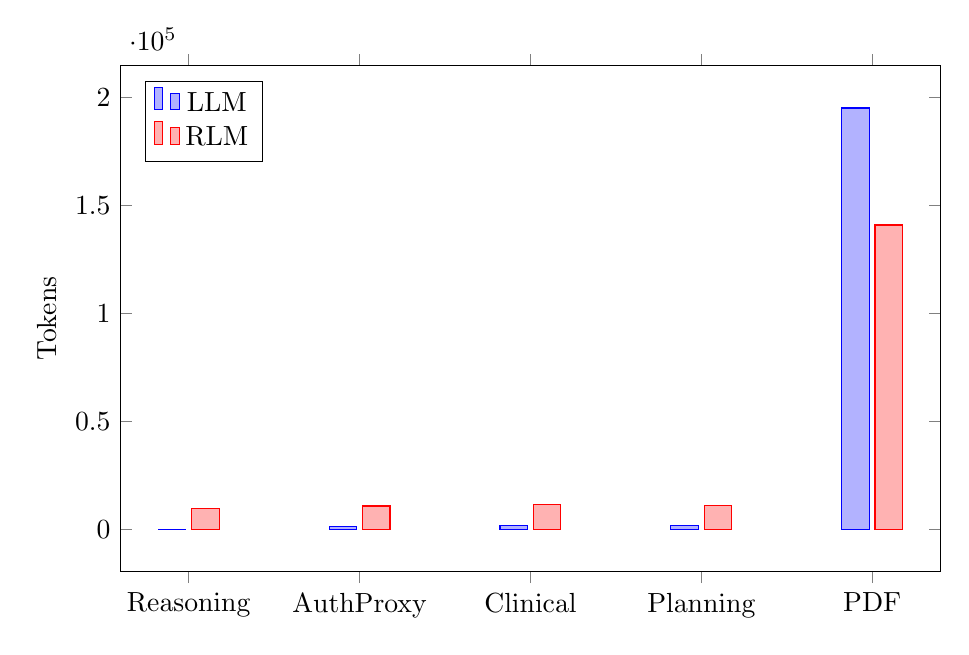
\begin{tikzpicture}
\begin{axis}[
    ybar,
    width=12cm,
    height=8cm,
    bar width=10pt,
    ylabel={Tokens},
    symbolic x coords={Reasoning,AuthProxy,Clinical,Planning,PDF},
    xtick=data,
    legend pos=north west,
]
\addplot coordinates {
    (Reasoning,270)
    (AuthProxy,1512)
    (Clinical,2124)
    (Planning,2144)
    (PDF,195109)
};
\addplot coordinates {
    (Reasoning,9650)
    (AuthProxy,11003)
    (Clinical,11771)
    (Planning,11216)
    (PDF,141006)
};
\legend{LLM,RLM}
\end{axis}
\end{tikzpicture}
\end{center}

\subsection{Latency Comparison}

\begin{center}
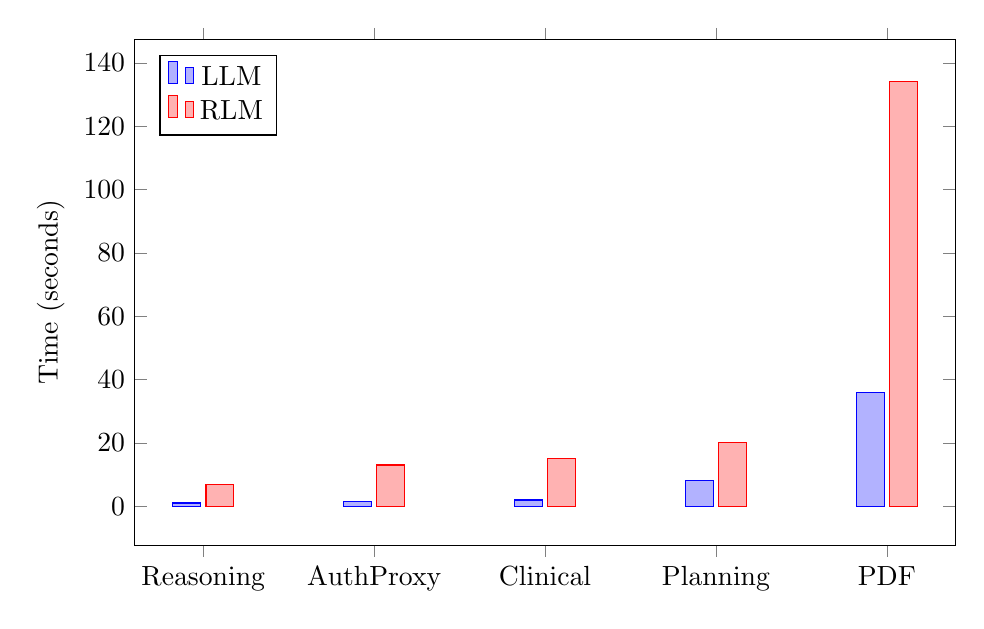
\begin{tikzpicture}
\begin{axis}[
    ybar,
    width=12cm,
    height=8cm,
    bar width=10pt,
    ylabel={Time (seconds)},
    symbolic x coords={Reasoning,AuthProxy,Clinical,Planning,PDF},
    xtick=data,
    legend pos=north west,
]
\addplot coordinates {
    (Reasoning,1)
    (AuthProxy,1.46)
    (Clinical,1.96)
    (Planning,8)
    (PDF,36)
};
\addplot coordinates {
    (Reasoning,6.78)
    (AuthProxy,13)
    (Clinical,15)
    (Planning,20)
    (PDF,134)
};
\legend{LLM,RLM}
\end{axis}
\end{tikzpicture}
\end{center}

\subsection{Efficiency Comparison}

Efficiency is approximated here as accuracy per token usage.

\begin{center}
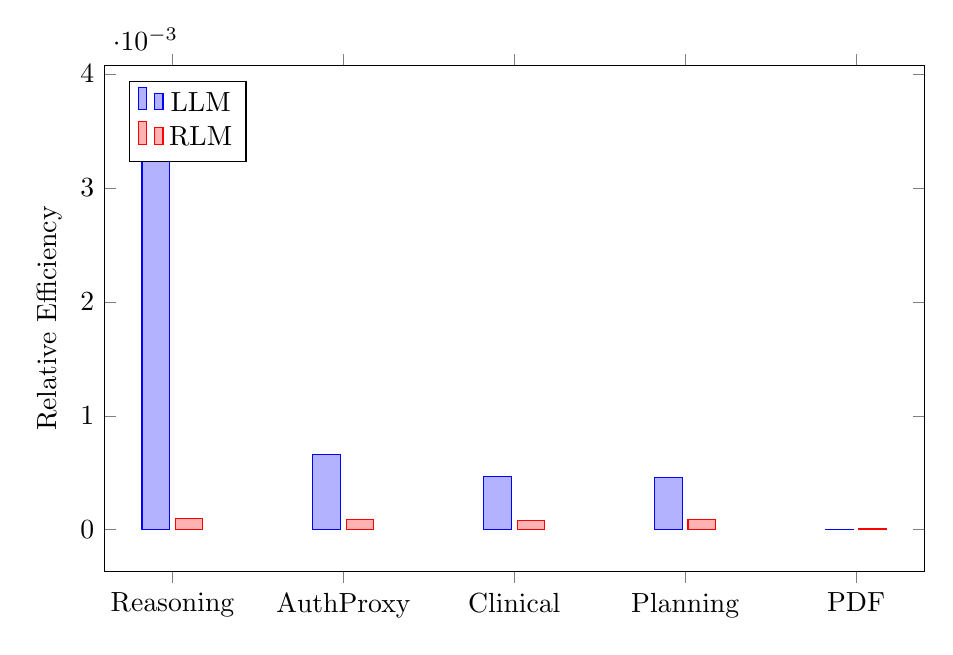
\begin{tikzpicture}
\begin{axis}[
    ybar,
    width=12cm,
    height=8cm,
    bar width=10pt,
    ylabel={Relative Efficiency},
    symbolic x coords={Reasoning,AuthProxy,Clinical,Planning,PDF},
    xtick=data,
    legend pos=north west,
]
\addplot coordinates {
    (Reasoning,0.0037)
    (AuthProxy,0.00066)
    (Clinical,0.00047)
    (Planning,0.00046)
    (PDF,0.000005)
};
\addplot coordinates {
    (Reasoning,0.0001)
    (AuthProxy,0.00009)
    (Clinical,0.00008)
    (Planning,0.00009)
    (PDF,0.000007)
};
\legend{LLM,RLM}
\end{axis}
\end{tikzpicture}
\end{center}

\section{RLM-Specific Behavioral Findings}

\subsection{Strategy Selection Limitations}

RLM often chose suboptimal strategies, such as:

\begin{itemize}
    \item relying on \texttt{llm\_query} instead of grounded retrieval
    \item ignoring available tools unless explicitly forced
\end{itemize}

\subsection{Tool Use vs Autonomy}

\begin{itemize}
    \item Tool use worked when explicitly enforced.
    \item Autonomous tool selection was unreliable.
\end{itemize}

\subsection{Context Handling}

\begin{itemize}
    \item RLM could operate directly on context when explicitly instructed.
    \item It did not reliably execute effective retrieval strategies on its own.
\end{itemize}

\subsection{Directed vs Autonomous Execution}

\begin{center}
\begin{tabular}{|l|l|}
\hline
Mode & Outcome \\
\hline
Autonomous RLM & Unreliable / failure-prone \\
Constrained RLM & Successful but rigid \\
\hline
\end{tabular}
\end{center}

\section{Conclusion}

Across all tasks:

\begin{itemize}
    \item Direct LLM prompting provided the best balance of latency, token efficiency, and reliability.
    \item RLM added substantial computational overhead without consistent improvements in output quality.
    \item RLM worked best as a controlled execution framework rather than an autonomous reasoning system.
\end{itemize}

The results show that, in this setup, RLM is not yet a strong solution for autonomous long-context reasoning or retrieval. It can still be useful when tightly constrained and instrumented for controlled execution and debugging.

\end{document}
